%\documentstyle{article}
\documentclass[10pt,letterpaper]{article}
\usepackage{tikz}
\usetikzlibrary{arrows}
\usetikzlibrary{graphs, graphs.standard, quotes}% quotes library is for the [""] edges
\oddsidemargin 0.15in
\textwidth 6.25in
\topmargin-0.75in
\textheight 9.5in
\headsep 0.6in
%\input epsf
\usepackage{graphicx}
\begin{document}
\begin{tabular}{ll}
{\bf Drexel University}  \\
{\bf Department of Computer Science } \\
{\bf CS 521: Data Structures and Algorithms}& \hspace{1in}{\it Summer 2022} \\
\hline
\end{tabular}
\vspace{0.75 in}
\begin{center}
\begin{LARGE}{Final  Exam} \end{LARGE}
\end{center}
\vspace{0.5in }
\begin{itemize}
\item This exam is intended to test your knowledge, therefore it is closed to outside sources (book, internet, and peers).
\item For an extra 5 points return your exam with a .tex file and a pdf built from compiled text. You can also write and scan your answers neatness counts!
\item Show  your work, as  partial credit will  be given. You  will be
  graded not only on the correctness of your answer, but also on the
  clarity with which you express it. Be neat!
\item YOu can earn up to 115 points on this exam but the grade will be out of 100.
\item {\large \bf Good Luck!}
\end{itemize}
\begin{center}
\begin{tabular}{||l|c|c||}
\hline
\hline
{\sc Problem} & {\sc Points} & {\sc Score}\\
\hline
\hline
{1} & 20 & \\
\hline
{2.} & 30 & \\
\hline
{3.} & 20 & \\
\hline
{4.} & 20 & \\
\hline
{5.} & 20 & \\
\hline
{Latex.} & 5 & \\
\hline
\hline
{\sc Total} & 115 & \\
\hline
\hline
\end{tabular}
\end{center}
\newpage



\begin{itemize}
\item[{\bf Question 1.}] Each recurrence below solves to one of the following:
\end{itemize}
$$ a.\Theta(\log n) \ \ \ b.\Theta(n)\ \ \ c.\Theta(n\log n)\ \ \
d.\Theta(n^2)\ \ \ e.\Theta(n^3) \ \ \ f.\Theta(3^{n/3})\ \ \
g.\Theta(5^{n/3})\ \ \ h.\Theta(2^{n}).$$
For each case, write down the label of the correct solution. Assume
the base case of  $T (n) = \Theta(1)$ when $n \le 3$. Show your work (master method, induction etc) \\ 

\begin{itemize}
\item[{a)}]  $T (n) = 4T (n/4) + 4n + 4$. 
\item[Ans: ] As T(n) looks similar to the T(n) = aT ($\frac{n}{b}$) + f(n)\\
so using the masters theorem we can solve this problem\\
where a=4,\\
b=4,\\
$n^\log_{b} a$ = $n^\log_{4} 4 = n$\\
f(n) = 4n + 4\\
f(n) = O($n^\logb a)$\\
using master theorem case 1 applied here \\
T(n) = $\Theta(n^\log_{b} a)$\\
which is T(n) = $\theta(n)$\\

\item[{b)}] $T(n) = T(n/3) + 2T(n/4) + n$.
\item[Ans: ] this equation can be solved using recursive tree method\\
I did not know how to draw the tree here in perfect way thats why I am using the sequence letter first row only n then one time n/3 and 2 times n/4 and continue till end.\\

n $->$ n\\
n/3 - (n/3) n/4 - (n/4) n/4 - (n/4) $->$ 5n/6\\
n/$3^2$ n/12 n/12 n/12 n/$4^2$ n/$4^2$ n/$4^2$ n/12 n/$4^2$ n/$4^2$ $->$ 25n/36\\
up to ... n/$3^k$ till n/$4^k$\\

left weight will be $\log_{3} n$ and right weight will be $\log_{4} n$\\
thus the time complexity from the above process of recursive tree \\
T(n) = n + 5n/6 + $5^2n/6^2$ + ... $\log_{3} n $ times.\\
T(n) = n[$(5/6)^0+(5/6)^1+...\log_{3}n times$]\\
T(n) = O(n) \\
left and right weights are varies in constant \\
T(n) = $\theta(n)$\\

\item[{c)}] $T(n)=T(n-2)+n^2 +n$.   
\item[Ans: ] to solve this equation im going to use the substitution method\\
T(n) = T(n-4) + $(n-2)^2$ + (n-2) + $n^2$ + n\\
T(n) = T(n-6) + $(n-4)^2$ + (n-4) + $(n-2)^2$ + (n-2) + $n^2$ + n\\
T(n) = T(n-8) + $(n-6)^2$ + (n-6) + $(n-4)^2$ + (n-4) + $(n-2)^2$ + (n-2) + $n^2$ + n\\
up to ...\\
T(n) = T(n-n) + ($n-(n-2))^2$ + (n-(n-2)) + ... + $(n-2)^2$ + (n-2) + $n^2$ + n\\
T(n) = T(0) + ($2^2 + 4^2 + ... + (n-2)^2 + n^2$) + (2+4+...+(n-2) + n)\\
T(n) = T(0) + $2^2$ ($1^2 + 2^2 + ... + (n/2)^2$)+ 2[1+2+...+(n/2)]\\
T(n) = 0+4[n/2[n/2 +1][2n/2+1]/6]+2[n/2[n/2+1]/2]\\

T(n) = n(n+2)(n+1) / 6 + n(n+2) / 4\\
n(n+2)(n+1) / 6 = O($n^3)$ and n(n+2) / 4 = O($n^2)$\\
T(n) = O($n^3$) therefore \\
T(n) = $\theta n^3$\\

\end{itemize}

\newpage


\begin{itemize}
\item[{\bf Question 2.}]
Indicate for each pair of expressions $(A,B)$ in the table below, whether $A$ is $O, o, \Omega, \omega$ or $\Theta$ of $B$. Assume $K \ge 1, \epsilon > 0$, and $c > 1$ are constants. You can fill in the table below for your answer using just a Y or N. \\ \\
a)$lg^kn$ $n^\epsilon$ \\
here we can see this that the n grows faster than the log n as log is small value thats why this relation is Yes for Big O and small o relation.\\

b)$n^k$ $C^n$\\
in this equation A is polynomial and B is exponential from that we can specify this exponential grows faster than polynomial. so it is Yes for Big O and small o.\\

c) $\sqrt{n}$ $n^{sin(n)}$\\
sin n value oscillate between [1,1] and it cannot be upper and lower bound.\\
$n^{sin(n)}$ using $\sqrt{n}$ = $n^\frac{1}{2}$\\

d) $2^n$ $2^{n/2}$\\
$2^n$ grows faster than $2^{n/2}$ \\

= $2^{\frac{1}{2}} . {n}$\\

= $(\sqrt{2})^n$ \\

since 2 $>$ $\sqrt{2}$\\

e) $n^{lgc}$ $c^{lgn}$\\
this is property of logarithm $n^{lgc}$ = $c^{lgn}$\\

f) $lg(n!)$ $lg(n^n)$\\
since both side there is log we compare the inner function lets see first \\
n factorial will be 1,2,3,4,5..... up to n and \\
$n^n$  = $\frac{n.n.n.n.....n}{n times}$ \\

so $n^n$ grows faster than n factorial.\\

{\begin{tabular}{ |c|c|c|c|c|c|c|c|c| }
  \hline
   & $A$ & $B$ & $O$ & $o$ & $\Omega$ & $\omega$ & $\Theta$ \\
  \hline
  a. & $lg^kn$ & $n^\epsilon$  &$Yes$   &$Yes$   &$No$   &$No$   &$No$  \\ 
  \hline
  b. & $n^k$ & $C^n$  &$Yes$  &$Yes$  &$No$  &$No$  &$No$  \\ 
  \hline
  c.  & $\sqrt{n}$ & $n^{sin(n)}$  &$No$  &$No$  &$No$  &$No$  &$No$  \\ 
  \hline
  d. & $2^n$ & $2^{n/2}$  &$No$  &$No$  &$Yes$  &$Yes$  &$No$  \\ 
  \hline
  e. & $n^{lgc}$ & $c^{lgn}$ &$Yes$  &$No$  &$Yes$  &$No$  &$Yes$  \\ 
  \hline
  f. & $lg(n!)$ & $lg(n^n)$ &$Yes$  &$Yes$  &$Yes$  &$No$  &$Yes$  \\ 
  \hline
\end{tabular}}
\label{}
\end{itemize}


\newpage

\begin{itemize} 
\item[{\bf Question 3.}] For each of the following questions, you are expected to
  give a short answer that fits in the space provided for each
  question.
\begin{itemize}

\item[a)] In modern software development, a useful utility called {\em make} is usually employed to manage the compilation order of files. The problem is: you are given $n$ files that need to be compiled. For each file assume you know the set of other files that are dependant on it.  Some of the files can only compile when some other files have been compiled. Explain a strategy for doing this using the algorithms we discussed in this course you do not need to formally prove the running time.
\item[Ans: ] Even though the make command has a lot of knowledge already, as you will see, it is unable to construct your application on its own. A file describing the design of your application must be supplied to make. The makefile is the name of this file.\\

Today's developers frequently have the impression that they are developing a rocket ship that will be shot into a black hole. They put in a lot of effort to produce something amazing, but they never truly know if their customers will find it useful. \\

Modern software development trends: 
Software and IT teams typically use agile software development tools to transition code from development to production that interacts with customers. That is a lot of equipment! Continuous delivery can be extremely challenging and time-consuming for large, monolithic code bases. \\

Teams are constrained by monoliths because integrating various services and features can result in problems that are challenging to pinpoint, developers frequently lack a deep understanding of one another work, and lengthy build and test periods might cause a deployment to sputter. \\

However, according to our study, 71 percent of software and IT teams that employ a microservices structure believe it makes it simpler to test or deploy new features. That's because some of those crucial deployment functions are built directly into the platform when teams use platform-as-a-service. Small, autonomous teams may autonomously build, launch, and expand their services thanks to a microservices-based design.\\

Manual testing is done, CU/CD. The use of automated testing It's no secret that consumers in this day and age expect the technology they use to be continuously updated, and if it isn't, they will replace it. Over the past few years, how many iPhones have you owned? \\

Sadly, manual testing is one of the main reasons organizations can't ship "early and often": difficulties with manual testing affect 62 percent of teams and are caused by insufficient automated test coverage, additional manual processes, and a lack of build/deployment pipeline automation.\\

For an input number N\\
  | - If N is even, set N to N / 2\\
  | - If N is odd,  set N to 3*N + 1\\

$#include <stdio.h>$\\
$#include <stdlib.h>$\\
$#include "mat.h"$\\
int main(int argc, char **argv){\\
  if(argc $<$ 3){\\
    printf("usage: %s {nx} {x1 x2 ...} {ny} {y1 y2 ...}\n",argv[0]);\\
    exit(1);\\
  }
  int i,j;\\
  int nx = atoi(argv[1]);\\
  double *x = (double *) malloc(sizeof(double) * nx);\\
  for(i=0; i$<$nx; i++){\\
    x[i] = atof(argv[i+2]);\\
  }
  int ny = atoi(argv[2+nx]);\\
  double *y = (double *) malloc(sizeof(double) * ny);\\
  for(i=0; i$<$ny; i++){\\
    y[i] = atof(argv[i+3+nx]);\\
  }

  double **mat = outer_product(x,nx, y,ny);\\
  for(i=0; i$<$nx; i++){\\
    for(j=0; j$<$ny; j++){\\
      printf("%8.2f ",mat[i][j]);\\
    }
    printf("\n");\\
  }

  /* Free memory */\\
  free(x);\\
  free(y);\\
  free_matrix(mat, nx);\\
  return 0;\\
}
  
\reference The "make" Command and "Makefiles". - Ram Naraian, HackerEarth, August 31, 2022, https://www.hackerearth.com/practice/notes/the-make-command-and-makefiles/\\
CSCI 4061: HW01 Compiling C Programs, Makefiles, August 31, 2022, https://www-users.cse.umn.edu/~kauffman/4061/hw01.html\\

\item[b)] Consider an array $A[1...n]$ of integers in the range
  $1...n^2$. A number $a$ is a {\em heavy hitter} in $A$ if $a$ occurs
  in $A$ at least $n/2$ times.  Note that an array of size $n$ can
  have at most two heavy hitters. Give an $O(n\log n)$ algorithm that
  finds all heavy hitters in a given array $A$.
\item[Ans: ] It is now simple to determine the frequency of each element and may be completed in linear time if the array is sorted, which will cause all similar elements to line up next to one another.\\

Finding the Majority Element Algorithm\\
Initialize counter := 0, current := NULL.\\
[current stores the frontrunner for the majority element]\\
• For i = 1 to n:\\
– If counter == 0:\\
[In this case, there is no frontrunner.] 
∗ current := A[i]\\
∗ counter++\\
- else if A[i]==current:\\
[In this case, our confidence in the current frontrunner goes up.]\\
∗ counter++ \\
– else\\
[In this case, our confidence in the current frontrunner goes down.] 
∗ counter - -\\
Return current\\

class GFG{\\

// Function to find Majority element in an array it returns -1 if there is no majority element\\
public static int majorityElement(int[] arr, int n)\\
{
	
	// Sort the array in O(nlogn)\\
	Arrays.sort(arr);\\

	int count = 1, max_ele = -1,\\
		temp = arr[0], ele = 0,\\
			f = 0;\\

	for(int i = 1; i $<$= n; i++)\\
	{
		
		// Increases the count if the same element occurs otherwise starts counting new element\\
		if (temp == arr[i])\\
		{
			count++;\\
		}
		else\\
		{
			count = 1;\\
			temp = arr[i];\\
		}

		// Sets maximum count and stores maximum occurred element so far if maximum count becomes greater than n/2 it breaks out setting the flag\\
		if (max_ele $<$ count)\\
		{
			max_ele = count;\\
			ele = arr[i];\\

			if (max_ele $>$ (n / 2))\\
			{
				f = 1;\\
				break;\\
			}
		}
	}

	// Returns maximum occurred element if there is no such element, returns -1\\
	return (f == 1 $?$ ele : -1);\\
}

// Driver code\\
public static void main(String[] args)\\
{
	int arr[] = { 1, 1, 2, 1, 3, 5, 1 };\\
	int n = 7;\\

	System.out.println(majorityElement(arr, n));\\
}
}

Time Complexity: O(nlogn), Sorting requires O(n log n) time complexity.\\

int findMajorityElement(int All, int n)\\
sort(A, n)\\
int i = 1, count = 1\\
while (i$<$n)\\
{
while (i $<$ n and A[i] == A[i-1])\\
{
i=i+1\\
count = count + 1\\
}
if (count $>$ n/2)\\
return A[i-1]\\
count = 1\\
}
return -1\\

Time Complexity: Sorting the array + Linear Traversal (Each element is visited only once) = O(nlogn)+O(n) = O(nlogn)\\
Space Complexity: If we use merge sort, then O(n), else if we use Heap Sort, its 0(1)\\

 /reference CS168: The Modern Algorithmic Toolbox Lecture #2 ... - Stanford University, August 31, 2022, https://web.stanford.edu/class/cs168/l/l2.pdf\\
Majority Element, GeeksforGeeks, August 08, 2022, https://www.geeksforgeeks.org/majority-element/\\


\end{itemize}

\end{itemize}
\newpage

\begin{itemize}
\item[{\bf Question 4.}] Show that in any red-black tree $T$ with $n$ key-bearing
  nodes (i.e., not counting null leaves) there are at least $n/3$ black
  nodes (not counting leaves). [Hint: Show by induction on the
  subtrees that any subtree of $T$ with size $m$ and a black root has
  at least $m/3$ black nodes, and any subtree of $T$ with size $m$ and
  a red root has at least $(m-1)/3$ black nodes.]
 
\item[Ans: ] A red-black tree is a kind of self-balancing binary search tree where each node has an extra bit, and that bit is often interpreted as the color (red or black). These colors are used to ensure that the tree remains balanced during insertions and deletions. Although the balance of the tree is not perfect, it is good enough to reduce the searching time and maintain it around O(log n) time, where n is the total number of elements in the tree.\\

Rules That Every Red-Black Tree Follows: \\
Every node has a color either red or black.\\
The root of the tree is always black.\\
There are no two adjacent red nodes (A red node cannot have a red parent or red child).\\
Every path from a node (including root) to any of its descendants NULL nodes has the same number of black nodes.\\
All leaf nodes are black nodes.\\

This proof has two parts in each step. This is because, as the hint points, we must prove for both the case of a black root and a red root for each subtree.\\

Base case:\\
a. 1 black root with a child (red in this case): 1≥1/3. We have 2 nodes --one being the root and black, and the other node can being red. If the child is black the inequality is also preserved $2>=1/3$.\\

b. 1 red root and a child: 1>=3. We have 2 nodes here as well. One being red (the
root), and the other being black. This is because by definition of a red- black tree, a red node must have black children. We are done with our base case.\\

Inductive Hypothesis\\
a. Inductive Hypothesis: Assume that for all subtrees with size 1<x<m with a black root, there are at least x/3 black nodes.\\
b. Inductive Hypothesis: Assume that for all subtrees with size 1<x<m with a red
root, there are at least x-1/3 black nodes.\\
We want to show how we can take an arbitrary red-black subtree of size m, remove something from the subtree to obtain a small enough tree to apply the inductive hypothesis and complete the proof algebraically.\\

Proof:\\
a. Consider any red-black subtree T of size m with a black root. Then the subtree must have at least one child node. This is because if it does not, then trivially it satisfies the inequality.\\
Consider the subtree T’ obtained by removing the child node. Now T’ has m-1 nodes and our inductive hypothesis applies. This means that T’ has at least (m-1)/3 black nodes. We removed exactly 1 node from T to make T’, yet we cannot use that node to make our case since the node can either be red or black. But since we know the root to be black, it must be that T has at least (m-1+1)/3= m/3 black nodes completing our proof.\\
b. Consider any red-black subtree T of size m with a red root. Then the subtree must have a least one node (not including the root).\\
Consider the subtree T’ obtained by removing the child node which must be
black by definition of a red-black tree. Now T’ has m-1 nodes and our inductive hypothesis applies. This means that T’ has a least (m-1-1)/3 = (m-2)/3 black nodes. But since we removed exactly 1 black node from T to generate T’, it must be that T has (m-2+1)/3 = (m-1)/3 black nodes completing our proof.\\

\tikzset{
  treenode/.style = {align=center, inner sep=0pt, text centered,
    font=\sffamily},
  arn_n/.style = {treenode, circle, white, font=\sffamily\bfseries, draw=black,
    fill=black, text width=1.5em},% arbre rouge noir, noeud noir
  arn_r/.style = {treenode, circle, red, draw=red, 
    text width=1.5em, very thick},% arbre rouge noir, noeud rouge
  arn_x/.style = {treenode, rectangle, draw=black,
    minimum width=0.5em, minimum height=0.5em}% arbre rouge noir, nil
}

\begin{tikzpicture}[->,>=stealth',level/.style={sibling distance = 5cm/#1,
  level distance = 1.5cm}] 
\node [arn_n] {12}
    child{ node [arn_n] {5} 
            child{ node [arn_n] {3} 
            				child{ node [arn_x] {}}
							child{ node [arn_r] {4}}
            }
            child{ node [arn_r] {10}
			    child{ node [arn_n] {7}
				        child{ node [arn_r] {6}}
				        child{ node [arn_r] {8}}
							}
							child{ node [arn_n] {11}}
            }                            
    }
    child{ node [arn_n] {15}
            child{ node [arn_n] {13} 
							child{ node [arn_x] {}}
							child{ node [arn_r] {14}}
            }
            child{ node [arn_n] {17}
            }
		}
; 
\end{tikzpicture}
the above red-black tree is 13 key bearing nodes (not including null leaves) it consist of n/3 black nodes 13/3\\
=4.\\
means the graph should have atleast 4 black nodes which the condition is satisfies because the tree has 8 black nodes. 

induction by subtree:\\
\begin{tikzpicture}[->,>=stealth',level/.style={sibling distance = 5cm/#1,
  level distance = 1.5cm}] 
\node [arn_r] {12}
    child{ node [arn_n] {7} 
            child{ node [arn_r] {6} 
            }
            child{ node [arn_r] {8}
            }                            
    }
    child{ node [arn_n] {11}
		}
; 
\end{tikzpicture}

the above tree is started with red root node and size is 5 according to the question it has (5-1)/3 = 1 black nodes.
the condition is satisfy as it has 2 black nodes.

\begin{tikzpicture}[->,>=stealth',level/.style={sibling distance = 5cm/#1,
  level distance = 1.5cm}] 
\node [arn_n] {15}
    child{ node [arn_n] {13} 
            child{ node [arn_x] {} 
            }
            child{ node [arn_r] {14}
            }                            
    }
    child{ node [arn_n] {17}
		}
; 
\end{tikzpicture}

the above tree is stated with black root and size is 4 according to the question it has atleast 4/3 = black node hence the condition is satisfies as it has 3 black nodes. therefore all the statement and proof considered as correct.\\

\reference Red-Black Tree: Set 1 (Introduction), GeeksforGeeks, June 07, 2022, https://www.geeksforgeeks.org/red-black-tree-set-1-introduction-2/\\

\end{itemize}
\newpage 

\begin{itemize}
\item[{\bf Question 5.}] Let $G=(V,E)$ be an undirected, connected graph with weight
  function $w: E\rightarrow R$, and suppose that $|E|\ge |V|$. Let $T$
  be a minimum spanning tree of $G$ and, for any two vertices $u,v\in
  V$, let $\max[u,v]$ be an edge of maximum weight on the unique path
  between $u$ and $v$ in $T$.  Describe an $O(|V|^2)$-time algorithm
  that, given $T$, computes $\max[u,v]$ for all $u,v\in V$. \\
\item[Ans: ] 
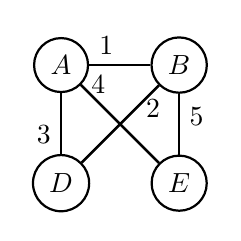
\begin{tikzpicture}[node distance={15mm}, thick, main/.style = {draw, circle}] 
\node[main] (1) {$A$}; 
\node[main] (2) [ right of=1] {$B$}; 
\node[main] (4) [ below of=1] {$D$}; 
\node[main] (5) [right of=4]{$E$}; 
\draw (1) -- (2) ; 
\draw (1) -- (4);
\draw (1) -- (5); 
\draw (2) -- (4);
\draw (2) -- (5);
\draw (1) -- node[midway, above right, sloped, pos=0] {1} (2); 
\draw (2) -- node[midway, above right, pos=0.7] {5} (5); 
\draw (1) -- node[midway, above left, pos=1] {3} (4); 
\draw (1) -- node[midway, right, pos=0] {4} (5); 
\draw (4) -- node[midway, right, pos=0.7] {2} (2); 
\end{tikzpicture} \\

EABD = 4,1,2 minimum spanning tree\\
DAEB = 3,4,1 second best minimum spanning tree\\
ABDE = 1,2,5 second best minimum spanning tree\\

Since any spanning tree has exactly $|V| - 1$ edges, any second-best minimum spanning tree must have at least one edge that is not in the (best) minimum spanning tree. If a second-best minimum spanning tree has exactly one edge, say $(x, y)$, that is not in the minimum spanning tree, then it has the same set of edges as the minimum spanning tree, except that $(x, y)$ replaces some edge, say $(u, v)$, of the minimum spanning tree. In this case, $T' = T - \{(u, v)\} \cup \{(x, y)\}$.\\

By performing a search from each vertex $u$ and limiting the edges visited to those of the spanning tree T, we can fill in max[u, v] for every u, v in V in $O(V^2)$ time. Whatever search method we use depth first, breadth first method.\\

Both the depth-first and breadth-first approaches will have pseudocode provided. We will use the max table itself to keep track of whether a vertex has been visited in a particular search, eliminating the requirement to compute d or f values. In particular, if and only if u = v or we have not yet visited vertex v in a search from vertex u, $max[u, v] = textNIL$. Also keep in mind that since we are visiting across edges in a spanning tree of an undirected graph, we can be sure that either a breadth-first or depth-first search from any vertex will reach all vertices.\\

Here's the breadth-first search approach:\\
BFS-FILL-MAX(G, T, w)\\
    let max be a new table with an entry max[u, v] for each u, v ∈ G.V\\
    for each vertex u ∈ G.V\\
        for each vertex v ∈ G.V\\
            max[u, v] = NIL\\
        Q = Ø\\
        ENQUEUE(Q, u)\\
        while Q != Ø\\
            x = DEQUEUE(Q)\\
            for each v ∈ G.Adj[x]\\
                if max[u, v] == NIL and v != u\\
                    if x == u or w(x, v) $>$ max[u, x]\\
                        max[u, v] = (x, v)\\
                    else max[u, v] = max[u, x]\\
                    ENQUEUE(Q, v)\\
    return max\\
    
Here's the depth-first search approach:\\
DFS-FILL-MAX(G, T, w)\\
    let max be a new table with an entry max[u, v] for each u, v ∈ G.V\\
    for each vertex u ∈ G.V\\
        for each vertex v ∈ G.V\\
            max[u, v] = NIL\\
        DFS-FILL-MAX-VISIT(G, u, u, max)\\
    return max\\
DFS-FILL-MAX-VISIT(G, u, x, max)\\
    for each vertex v ∈ G.Adj[x]\\
        if max[u, v] == NIL and v != u\\
            if x == u or w(x, v) $>$ max[u, x]\\
                max[u, v] = (x, v)\\
            else max[u, v] = max[u, x]\\
            DFS-FILL-MAX-VISIT(G, u, v, max)\\

For either approach, we are filling in $|V|$ rows of the $max$ table. Since the number of edges in the spanning tree is $|V| - 1$, each row takes $O(V)$ time to fill in. Thus, the total time to fill in the $max$ table is $O(V^2)$.

We can also solve this an algorithm that computes spike(P u,v) for all pairs u,v:\\
algorithm:\\
initialize a matrixS[u,v] to store the value of spike(Pu,v) for all u,v.\\
for each vertex u in T:\\
S[u,u]=0\\
mark u as visited.\\
while every vertex has not been visited:\\
for every vertex v neighbor of u:\\
S[u,v] = min(w(u,v)+S[u,u])\\
Mark v as visited\\
u=v\\
Since we proceed outside from u in a DFS manner, it takes only linear time for each vertex. Hence in total runs in $O(V^2)$ time.\\

\reference Algorithms Book Edition 4

\end{itemize}
\end{document}


